\subsection{Space-Only Modulation}
\label{subsec:space_only_modulation}

In the case of space-only modulation, a given pair of piezoelectric patches can be either in the short-circuit or open-circuit state.
For simplicity, we will refer to these states as ON and OFF, respectively.

Considering the ST cell as composed by three pairs of piezoelectric patches, three different configurations are analyzed:

\begin{itemize}
    \item OFF-OFF-OFF: all the shunt circuits are open;
    \item ON-ON-ON: all the shunt circuits are closed;
    \item OFF-OFF-ON: only the last shunt circuit is closed.
\end{itemize}

The mechanical properties of the system are computed so to obtain $EJ(x)$ and $\rho A(x)$, which are then used by the numerical methods to compute the dispersion diagram of the system.
In the following, the results of the numerical simulations are compared with the experimental data.

Both the TMM and PWEM are expected to exhibit some discrepancies with the experimental data at higher frequencies due to the hypothesis made in the theoretical model.
The Euler-Bernoulli beam theory that has been used in the theoretical model, is known to be a good approximation only for low-frequency excitations and small deformations.
Timošenko beam theory could have been a better choice, but it would have made the theoretical model more complex and the numerical simulations more computationally expensive.

Moreover, for the PWEM, a number of space and time harmonics equal to $P = 40$ and $Q = 1$ are considered, respectively.
The relative low number of space harmonics is expected to introduce some additional discrepancies with the experimental data, especially at higher frequencies.

\texttt{Comsol Multiphysics} is used as a valid reference to validate the experimental results given that internal losses and higher order modes are taken into account into its numerical solvers.


\paragraph{OFF-OFF-OFF}

The first case considered is the OFF-OFF-OFF configuration, where all the shunt circuits are open.
In this case, based on Equation \ref{eq:mechanical_admittance_shunted_piezoelectric_patch}, the piezo's mechanical admittance is given by:

\begin{equation}
    Y^{SU} = Y_1^D
\end{equation}

Figure \ref{fig:space_only_off_off_off}, shows the PWEM and experimental results, while the comparison between the TMM and Comsol Multiphysics is shown in Figure \ref{fig:space_only_off_off_off_comsol}.

\begin{figure}[H]
    \centering
    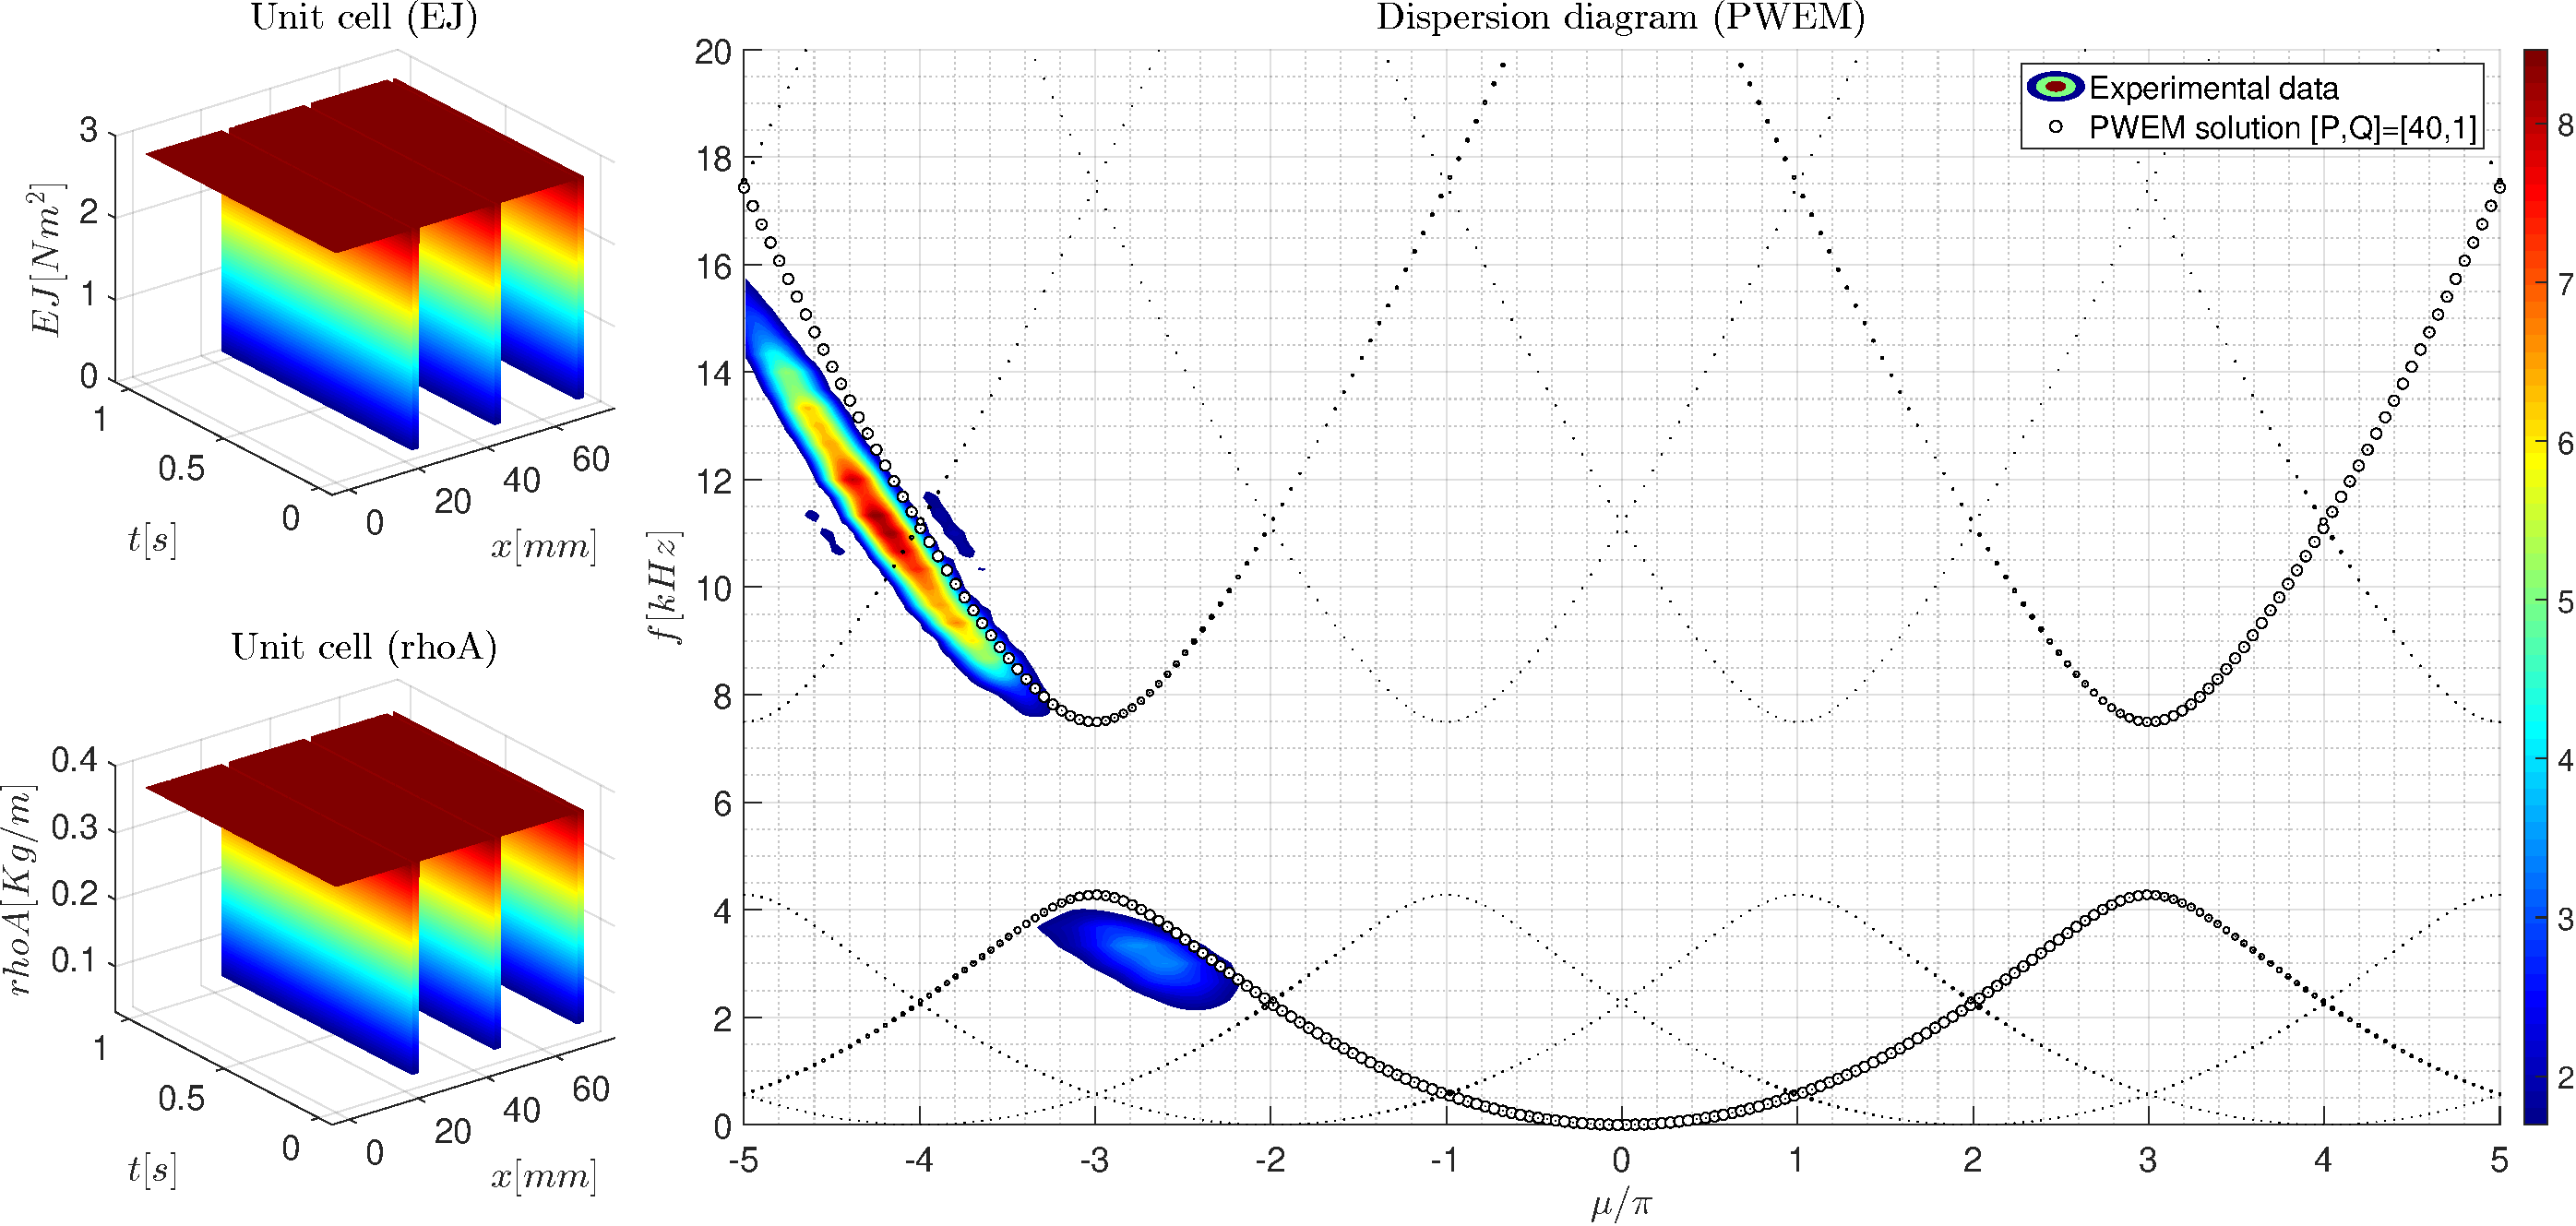
\includegraphics[width=\textwidth]{./img/MATLAB/PWEM_EXP OFF-OFF-OFF @0kHz.pdf}
    \caption{Band structure for the OFF-OFF-OFF configuration.}
    \label{fig:space_only_off_off_off}
\end{figure}

\begin{figure}[H]
    \centering
    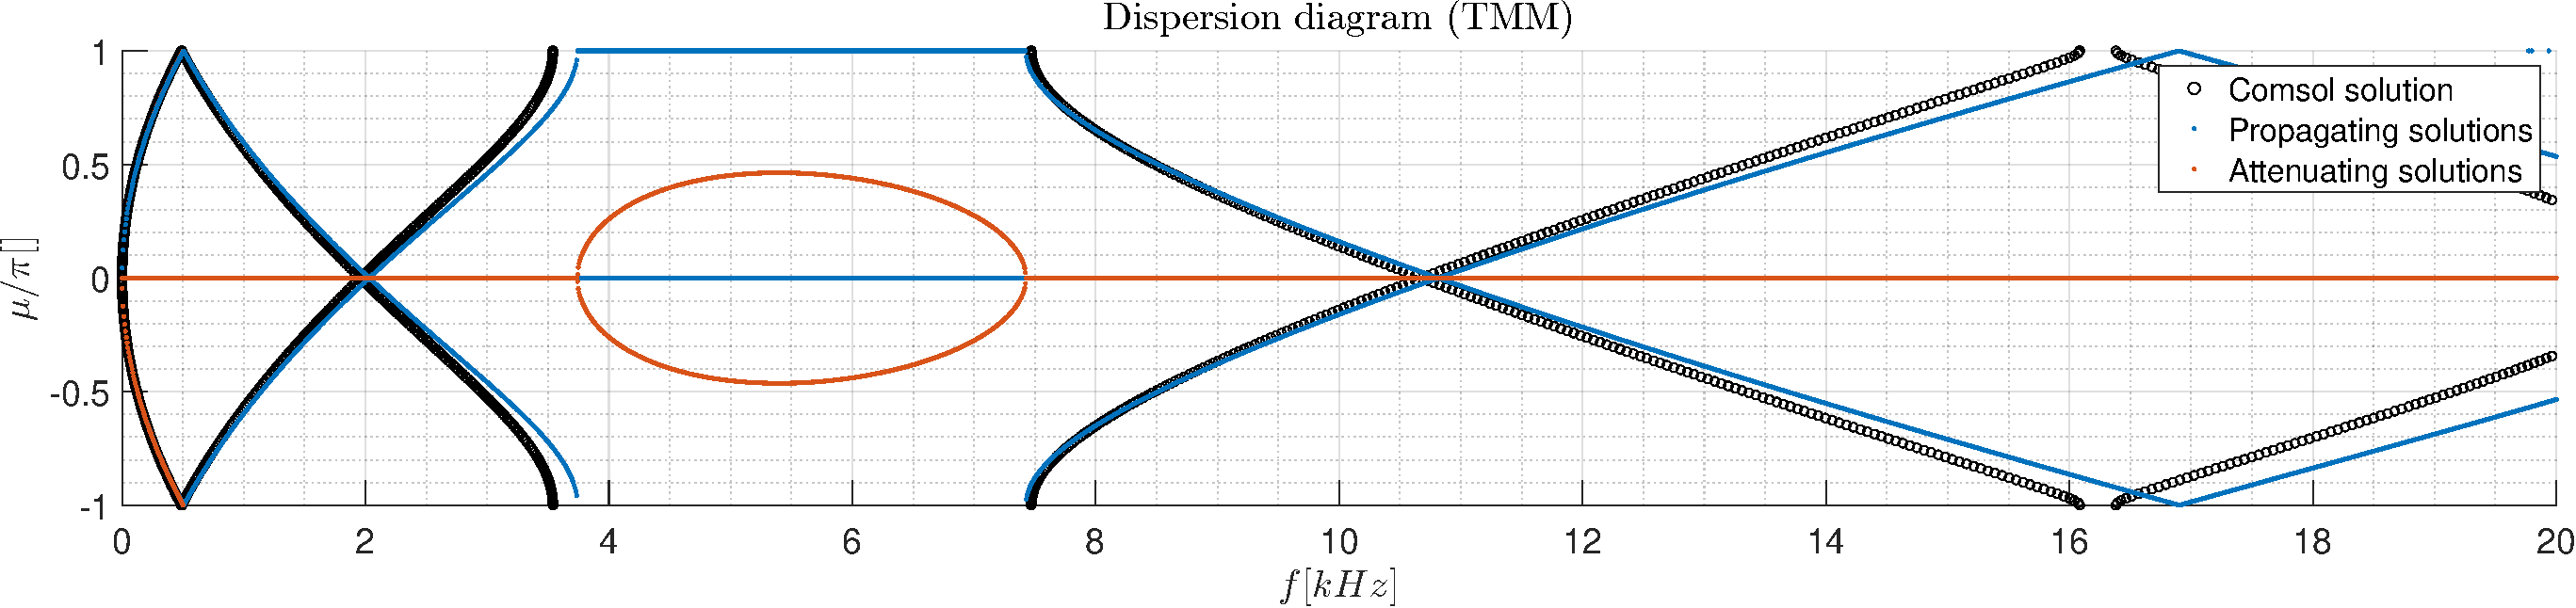
\includegraphics[width=\textwidth]{./img/MATLAB/TMM_COMSOL OFF-OFF-OFF @0kHz.pdf}
    \caption{Comparison between TMM and Comsol Multiphysics for the OFF-OFF-OFF configuration.}
    \label{fig:space_only_off_off_off_comsol}
\end{figure}

In the above figures, what has been suggested with the introductory considerations is confirmed.
Both the TMM and PWEM exhibit some discrepancies with the experimental data at higher frequencies.
However, their results are still in good agreement with the experimental data, being able to predict the band-gap position.

From the comparison between the TMM and Comsol Multiphysics, it can be seen that the TMM method underestimate the stiffness of the beam at higher frequencies, causing an upper shift of the dispersion diagram with respect to both the experimental data and the Comsol Multiphysics results.
Under the hypothesis that this offset is due to the Euler-Bernoulli assumption, we can state that the model can be considered valid for the analysis of the system.

In the case of the OFF-OFF-OFF configuration, the band gap of the structure is found at:

\begin{equation}
    f_{BG}^{OFF-OFF-OFF} = [3.8, 7.5] kHz
\end{equation}



\paragraph{ON-ON-ON}

The second case considered is the ON-ON-ON configuration, where all the shunt circuits are in the short-circuit state.
In this case, the piezo's mechanical admittance is given by:

\begin{equation}
    Y^{SU} = Y_1^E
\end{equation}

Figure \ref{fig:space_only_on_on_on}, shows the PWEM and experimental results, while the comparison between the TMM and Comsol Multiphysics is shown in Figure \ref{fig:space_only_on_on_on_comsol}.

\begin{figure}[H]
    \centering
    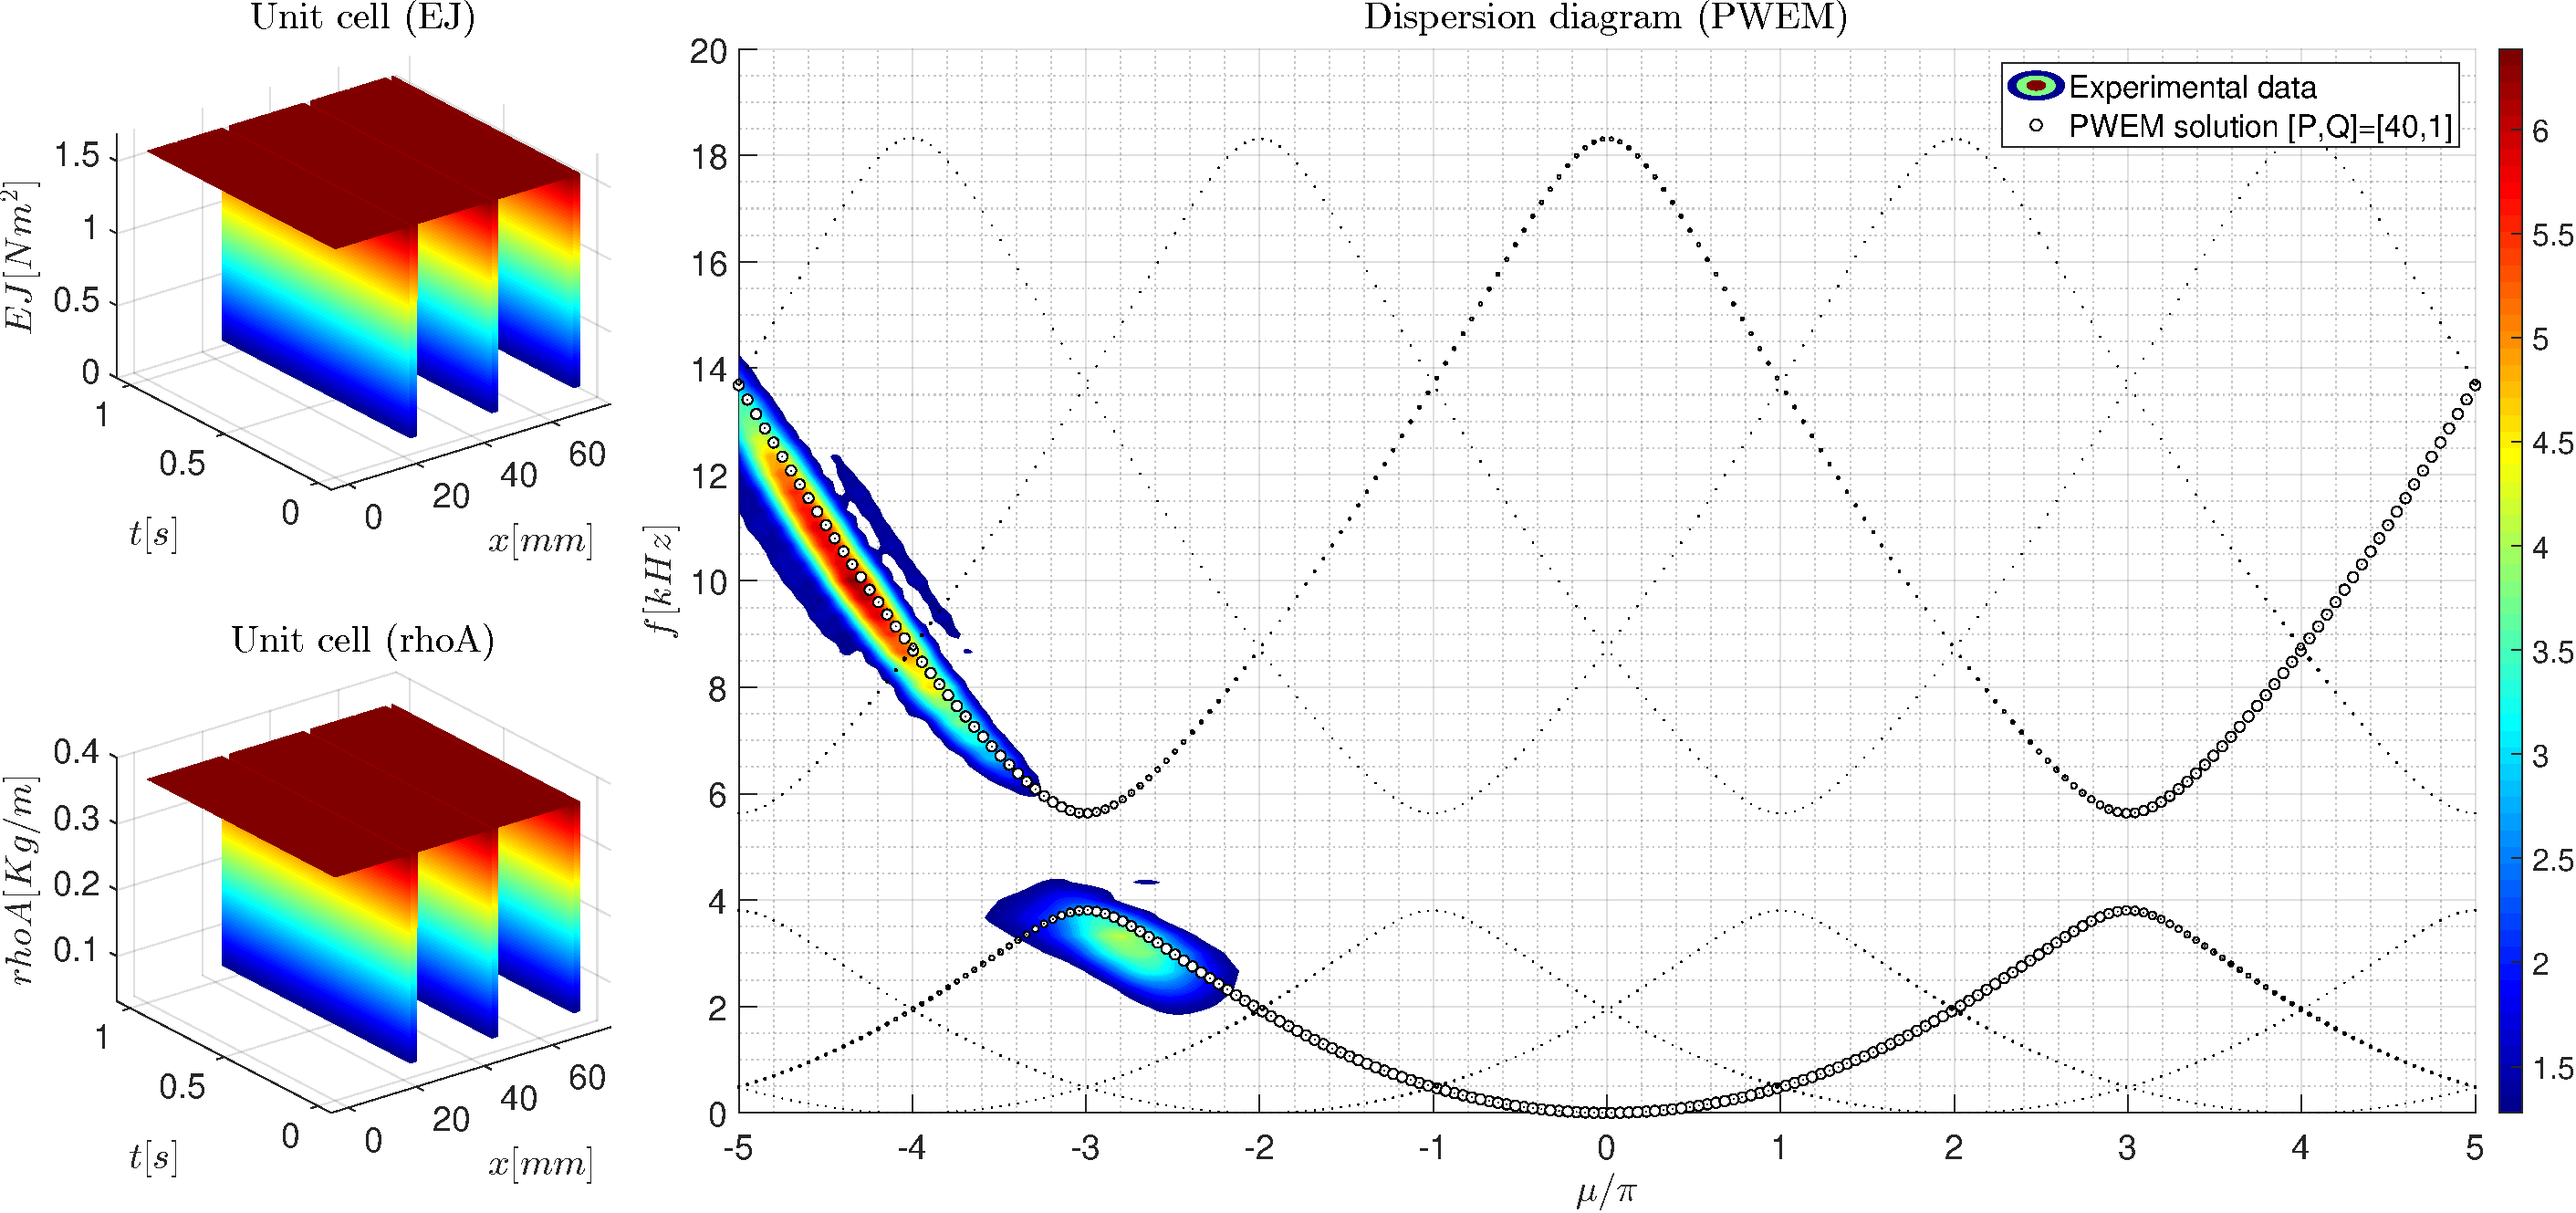
\includegraphics[width=\textwidth]{./img/MATLAB/PWEM_EXP ON-ON-ON @0kHz.pdf}
    \caption{Band structure for the ON-ON-ON configuration.}
    \label{fig:space_only_on_on_on}
\end{figure}

\begin{figure}[H]
    \centering
    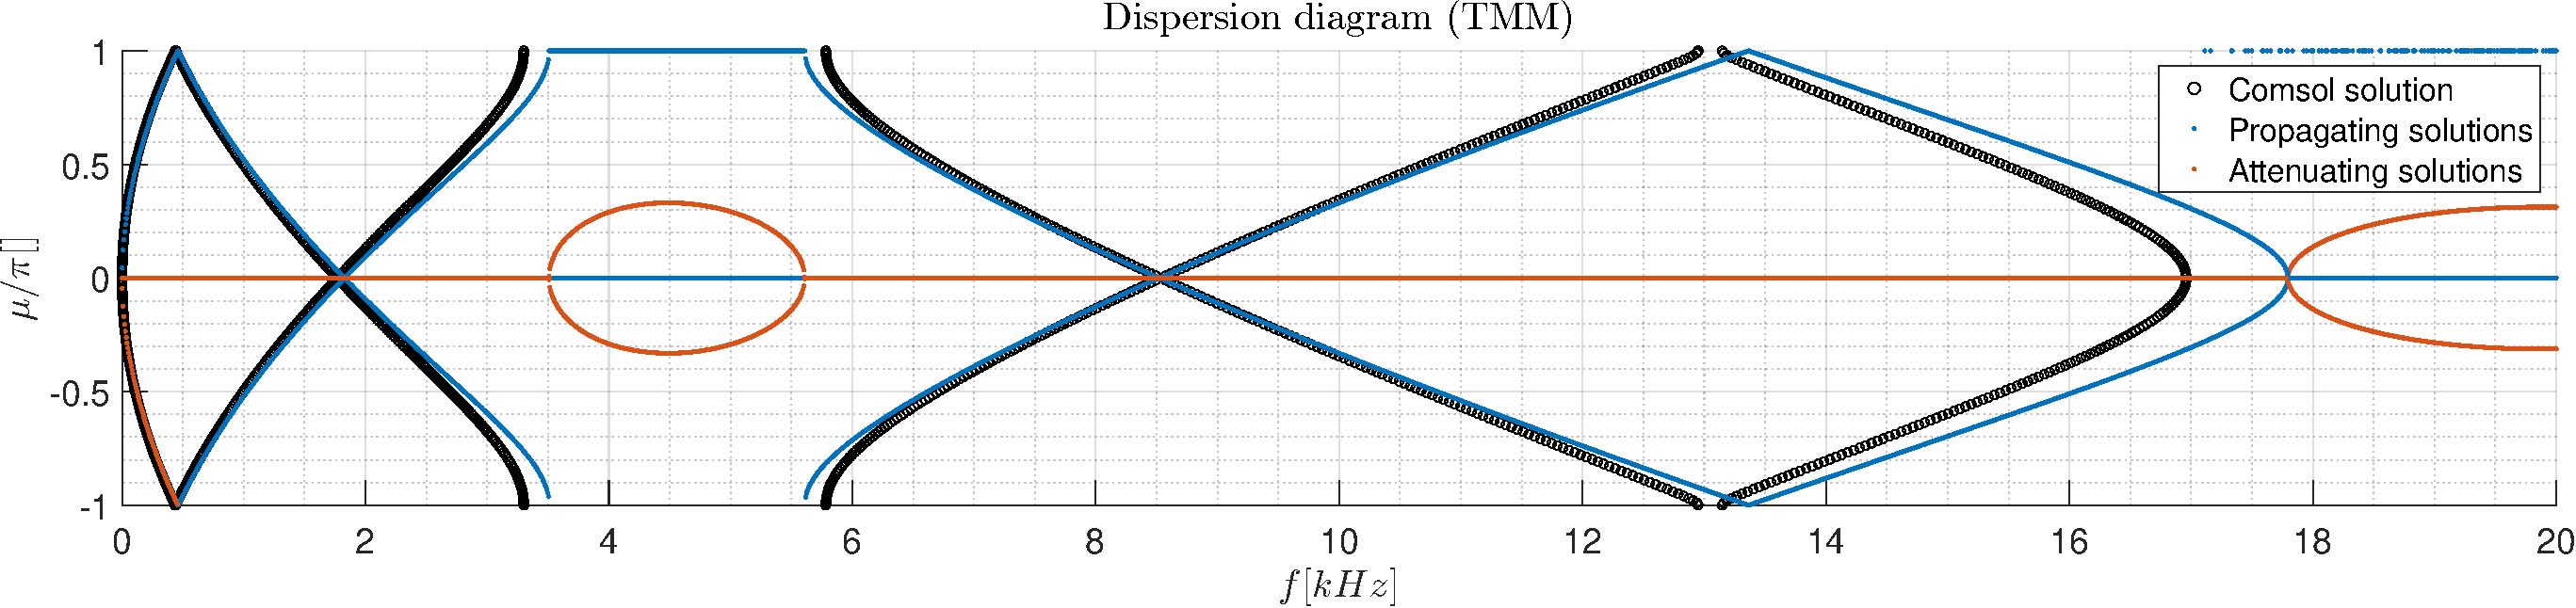
\includegraphics[width=\textwidth]{./img/MATLAB/TMM_COMSOL ON-ON-ON @0kHz.pdf}
    \caption{Comparison between TMM and Comsol Multiphysics for the ON-ON-ON configuration.}
    \label{fig:space_only_on_on_on_comsol}
\end{figure}

Similar consideration as before can be done about the discrepancy between the numerical methods and the experimental data.
Comsol Multiphysics is again used as a reference to validate the experimental results.

With respect to the ON-ON-ON configuration, a shift of the band-gap towards lower frequencies is observed:

\begin{equation}
    f_{BG}^{ON-ON-ON} = [3.4, 5.6] kHz
\end{equation}

This shift is due to the fact that the piezoelectric patches are in the short-circuit state, which results in a lower effective stiffness of the beam section.
Having a lower effective stiffness is equivalent to state that the speed of the travelling wave is lower, which results in a lower frequency of the band-gap.



\paragraph{ON-OFF-OFF}

The last case considered regarding the space-only modulation is the ON-OFF-OFF configuration, where only the first shunt circuit is closed and the other two are open.

It's intuitive to understand that the mechanical admittance is no more the same for the three piezoelectric patches.
This will introduce additional sources of dispersion in the system, which will result in higher number of band-gaps visible in the same frequency range.

Figure \ref{fig:space_only_on_off_off}, shows the PWEM and experimental results, while the comparison between the TMM and Comsol Multiphysics is shown in Figure \ref{fig:space_only_on_off_off_comsol}.

\begin{figure}[H]
    \centering
    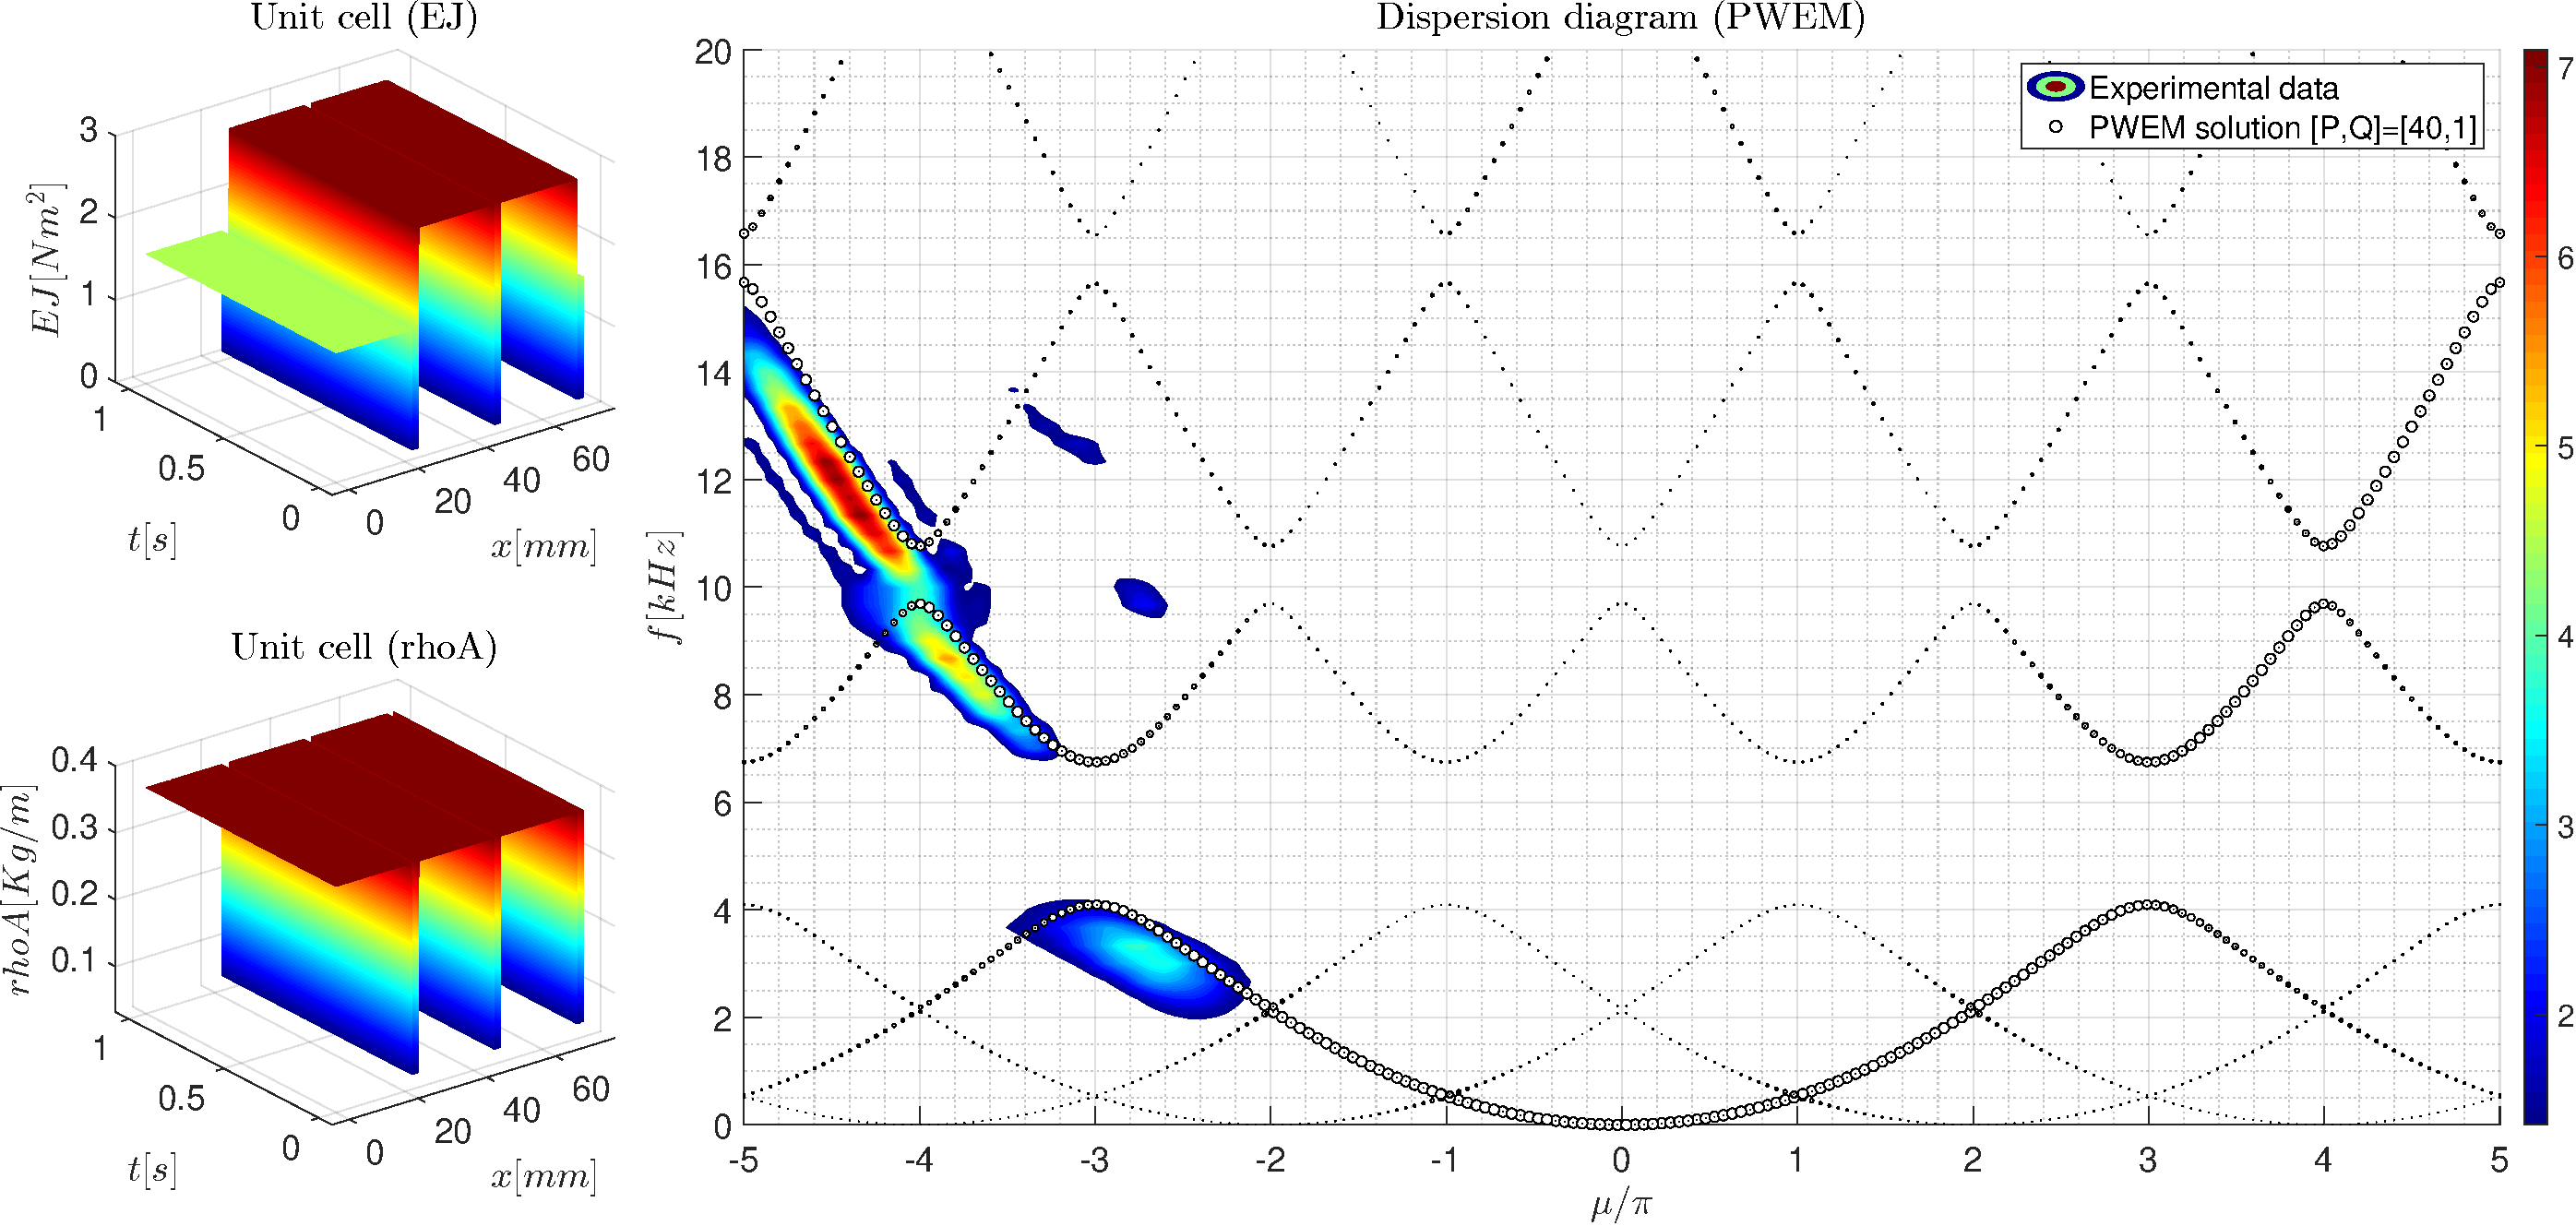
\includegraphics[width=\textwidth]{./img/MATLAB/PWEM_EXP ON-OFF-OFF @0kHz.pdf}
    \caption{Band structure for the ON-OFF-OFF configuration.}
    \label{fig:space_only_on_off_off}
\end{figure}

\begin{figure}[H]
    \centering
    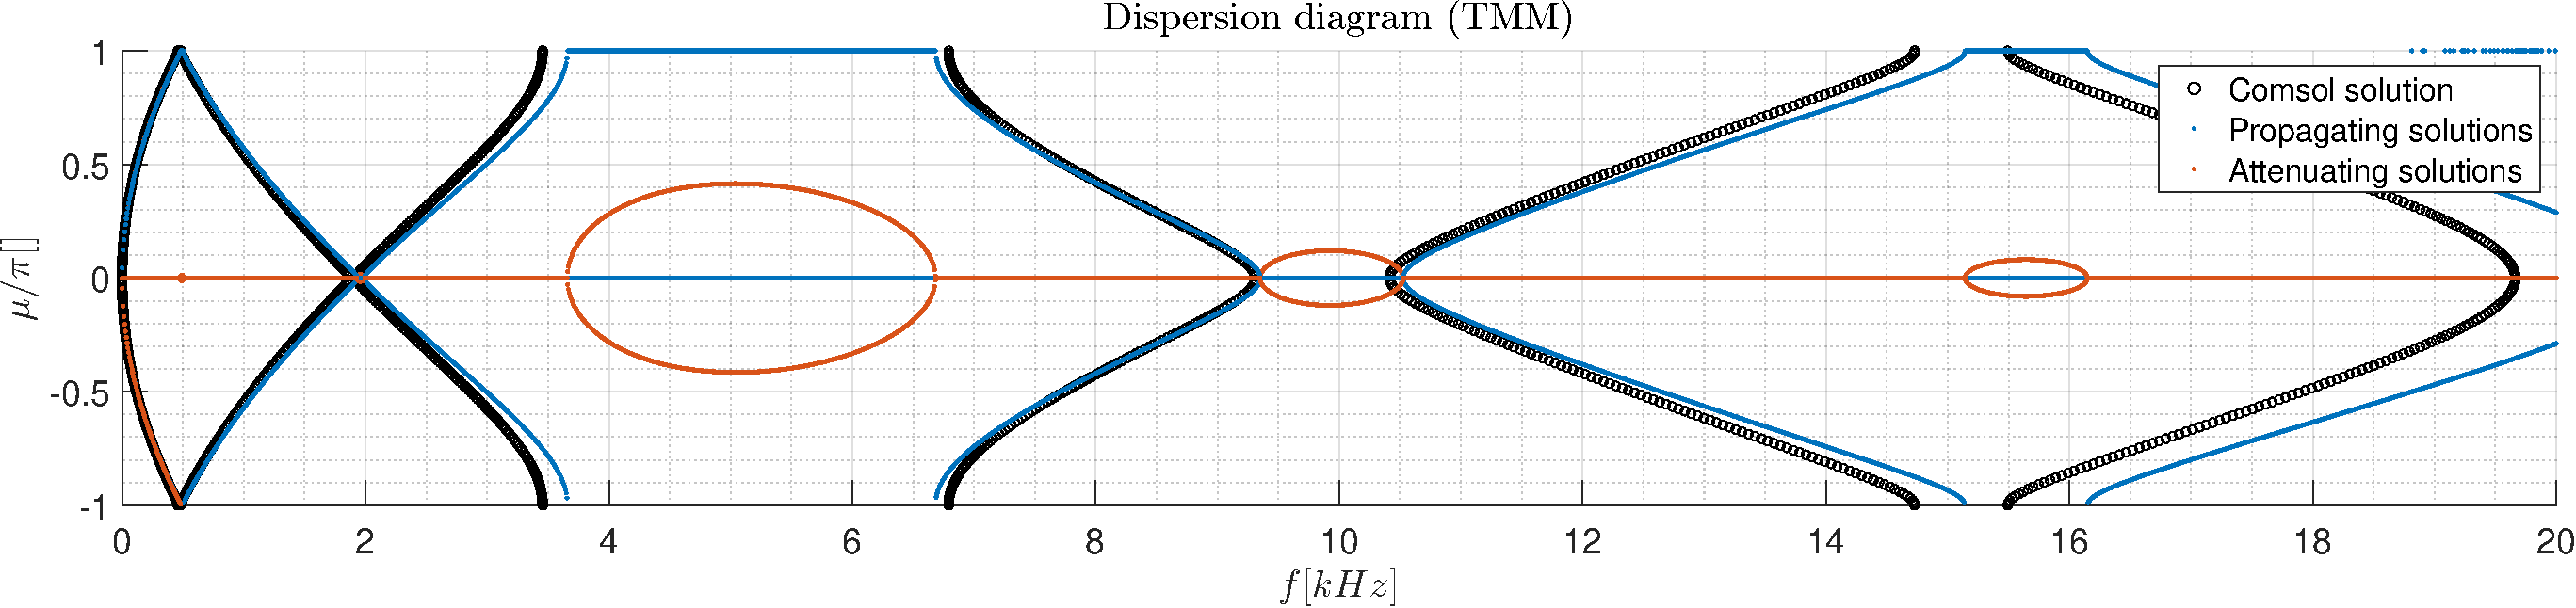
\includegraphics[width=\textwidth]{./img/MATLAB/TMM_COMSOL ON-OFF-OFF @0kHz.pdf}
    \caption{Comparison between TMM and Comsol Multiphysics for the ON-OFF-OFF configuration.}
    \label{fig:space_only_on_off_off_comsol}
\end{figure}

As a confirmation of the previous considerations, the band structure of the ON-OFF-OFF configuration shows a higher number of band-gaps in the same frequency range.

The band gap of the structure are now found at:

\begin{equation}
    \begin{aligned}
        f_{BG1}^{ON-OFF-OFF} & = [3.5, 6.7] kHz   \\
        f_{BG2}^{ON-OFF-OFF} & = [9.3, 10.4] kHz  \\
        f_{BG3}^{ON-OFF-OFF} & = [14.7, 15.5] kHz
    \end{aligned}
\end{equation}
